% m1_demo_grid.tex  the model in one picture: a 5 x 5 piece of map
% and the chance of each event in a short time dt.
%
% Compile:  pdflatex m1_demo_grid.tex     (or upload to Overleaf)
% PNG:      pdftoppm -png -r 220 -singlefile m1_demo_grid.pdf m1_demo_grid
%
% Made by tools/make_demo_grid.py; cell colours are written in below.
\documentclass[border=10pt]{standalone}
\usepackage{amsmath}
\usepackage{booktabs}
\usepackage{array}
\usepackage{colortbl}
\usepackage{tikz}
\usetikzlibrary{arrows.meta, calc}

\definecolor{ink}{HTML}{1F2937}
\definecolor{ink2}{HTML}{4B5563}
\definecolor{rule}{HTML}{D1D5DB}
\definecolor{birth}{HTML}{2F855A}
\definecolor{death}{HTML}{9C4221}
\definecolor{hopout}{HTML}{DD6B20}
\definecolor{hopin}{HTML}{2B6CB0}
\definecolor{nothing}{HTML}{6B7280}

\tikzset{
  hop/.style = {-{Stealth[length=2.6mm, width=2.2mm]}, line width=1.6pt},
  qlab/.style = {font=\small, anchor=north west, inner sep=0pt},
}

\begin{document}
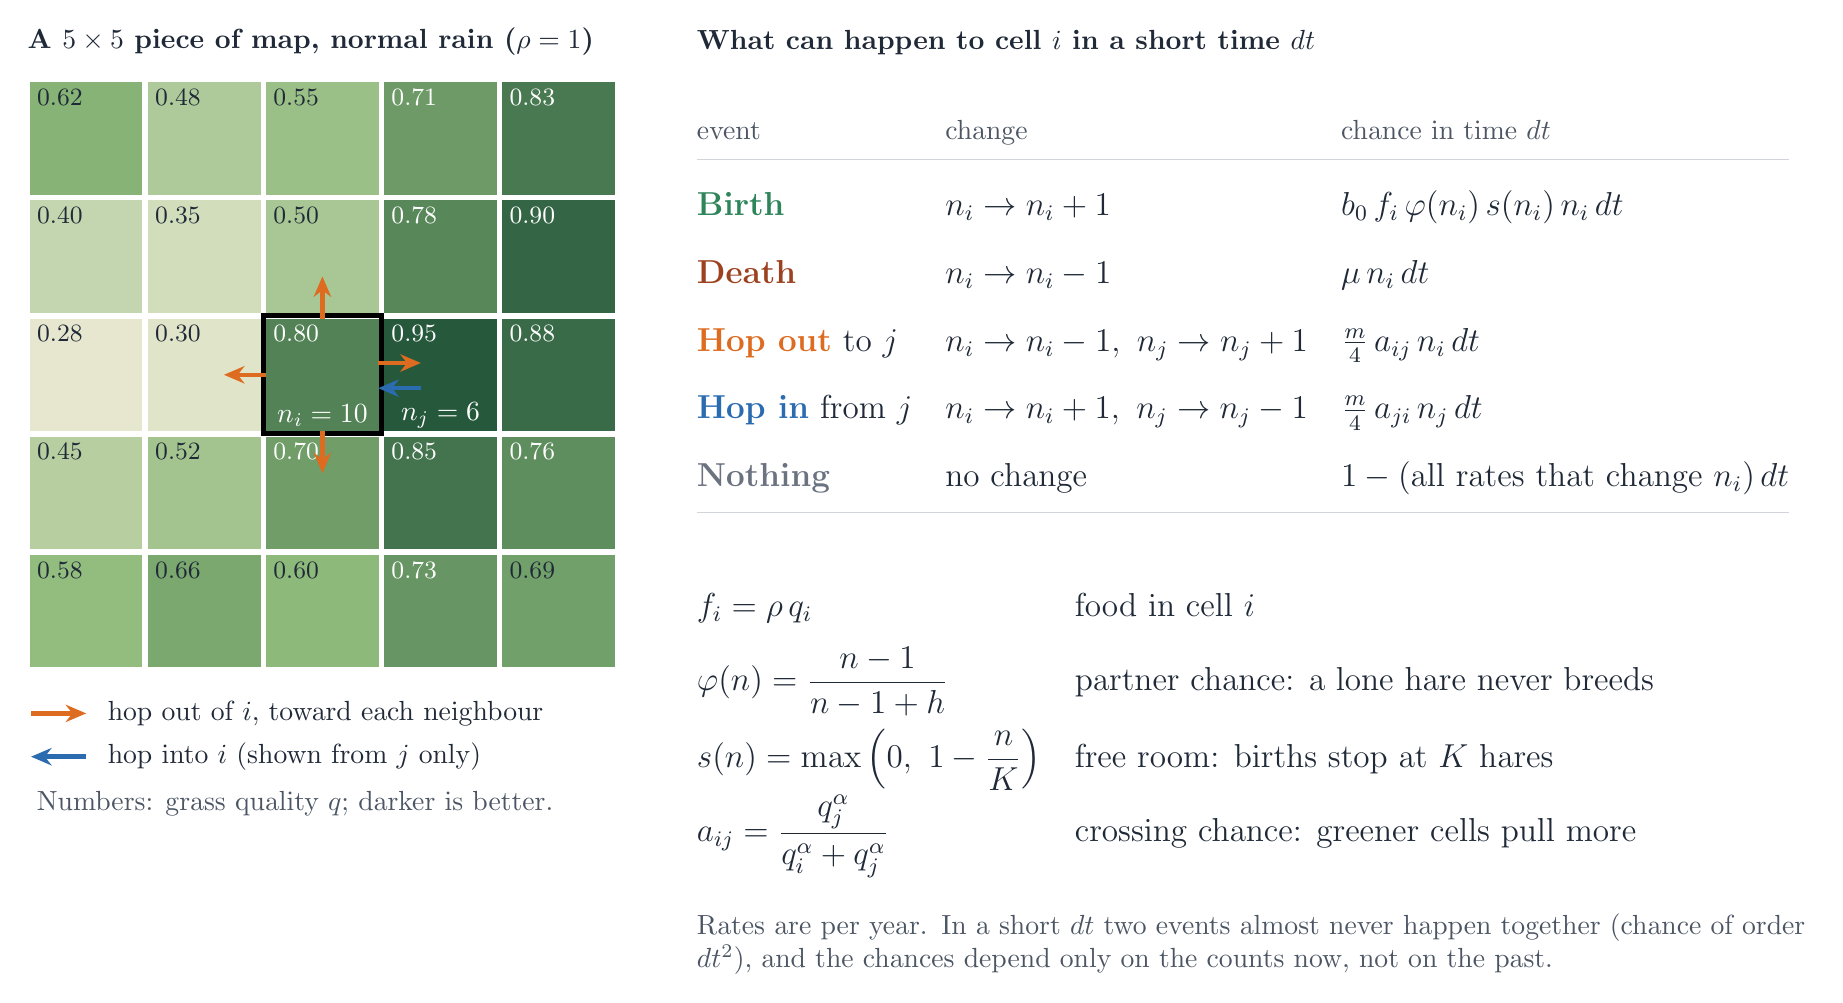
\begin{tikzpicture}[text=ink, font=\large]

% ---- the 5 x 5 grid; numbers are grass quality q -------------------
\node[font=\bfseries, anchor=south west, inner sep=0pt] at (0, 0.3)
  {A $5\times 5$ piece of map, normal rain ($\rho = 1$)};
\definecolor{q00}{HTML}{87B376}
\fill[q00] (0.035, -1.465) rectangle (1.465, -0.035);
\node[qlab, text=ink] at (0.120, -0.120) {0.62};
\definecolor{q01}{HTML}{AECA9A}
\fill[q01] (1.535, -1.465) rectangle (2.965, -0.035);
\node[qlab, text=ink] at (1.620, -0.120) {0.48};
\definecolor{q02}{HTML}{9BC087}
\fill[q02] (3.035, -1.465) rectangle (4.465, -0.035);
\node[qlab, text=ink] at (3.120, -0.120) {0.55};
\definecolor{q03}{HTML}{6D9A66}
\fill[q03] (4.535, -1.465) rectangle (5.965, -0.035);
\node[qlab, text=white] at (4.620, -0.120) {0.71};
\definecolor{q04}{HTML}{497951}
\fill[q04] (6.035, -1.465) rectangle (7.465, -0.035);
\node[qlab, text=white] at (6.120, -0.120) {0.83};
\definecolor{q10}{HTML}{C4D6AF}
\fill[q10] (0.035, -2.965) rectangle (1.465, -1.535);
\node[qlab, text=ink] at (0.120, -1.620) {0.40};
\definecolor{q11}{HTML}{D2DDBC}
\fill[q11] (1.535, -2.965) rectangle (2.965, -1.535);
\node[qlab, text=ink] at (1.620, -1.620) {0.35};
\definecolor{q12}{HTML}{A9C794}
\fill[q12] (3.035, -2.965) rectangle (4.465, -1.535);
\node[qlab, text=ink] at (3.120, -1.620) {0.50};
\definecolor{q13}{HTML}{58875A}
\fill[q13] (4.535, -2.965) rectangle (5.965, -1.535);
\node[qlab, text=white] at (4.620, -1.620) {0.78};
\definecolor{q14}{HTML}{346645}
\fill[q14] (6.035, -2.965) rectangle (7.465, -1.535);
\node[qlab, text=white] at (6.120, -1.620) {0.90};
\definecolor{q20}{HTML}{E6E7CE}
\fill[q20] (0.035, -4.465) rectangle (1.465, -3.035);
\node[qlab, text=ink] at (0.120, -3.120) {0.28};
\definecolor{q21}{HTML}{E0E4C9}
\fill[q21] (1.535, -4.465) rectangle (2.965, -3.035);
\node[qlab, text=ink] at (1.620, -3.120) {0.30};
\definecolor{q22}{HTML}{528256}
\fill[q22] (3.035, -4.465) rectangle (4.465, -3.035);
\node[qlab, text=white] at (3.120, -3.120) {0.80};
\definecolor{q23}{HTML}{26583C}
\fill[q23] (4.535, -4.465) rectangle (5.965, -3.035);
\node[qlab, text=white] at (4.620, -3.120) {0.95};
\definecolor{q24}{HTML}{3A6B48}
\fill[q24] (6.035, -4.465) rectangle (7.465, -3.035);
\node[qlab, text=white] at (6.120, -3.120) {0.88};
\definecolor{q30}{HTML}{B7CEA1}
\fill[q30] (0.035, -5.965) rectangle (1.465, -4.535);
\node[qlab, text=ink] at (0.120, -4.620) {0.45};
\definecolor{q31}{HTML}{A3C48F}
\fill[q31] (1.535, -5.965) rectangle (2.965, -4.535);
\node[qlab, text=ink] at (1.620, -4.620) {0.52};
\definecolor{q32}{HTML}{709D68}
\fill[q32] (3.035, -5.965) rectangle (4.465, -4.535);
\node[qlab, text=white] at (3.120, -4.620) {0.70};
\definecolor{q33}{HTML}{43744E}
\fill[q33] (4.535, -5.965) rectangle (5.965, -4.535);
\node[qlab, text=white] at (4.620, -4.620) {0.85};
\definecolor{q34}{HTML}{5E8D5E}
\fill[q34] (6.035, -5.965) rectangle (7.465, -4.535);
\node[qlab, text=white] at (6.120, -4.620) {0.76};
\definecolor{q40}{HTML}{93BC7F}
\fill[q40] (0.035, -7.465) rectangle (1.465, -6.035);
\node[qlab, text=ink] at (0.120, -6.120) {0.58};
\definecolor{q41}{HTML}{7BA86F}
\fill[q41] (1.535, -7.465) rectangle (2.965, -6.035);
\node[qlab, text=ink] at (1.620, -6.120) {0.66};
\definecolor{q42}{HTML}{8DB97A}
\fill[q42] (3.035, -7.465) rectangle (4.465, -6.035);
\node[qlab, text=ink] at (3.120, -6.120) {0.60};
\definecolor{q43}{HTML}{679563}
\fill[q43] (4.535, -7.465) rectangle (5.965, -6.035);
\node[qlab, text=white] at (4.620, -6.120) {0.73};
\definecolor{q44}{HTML}{72A06A}
\fill[q44] (6.035, -7.465) rectangle (7.465, -6.035);
\node[qlab, text=ink] at (6.120, -6.120) {0.69};
% ---- cell i (black frame) and its right neighbour j ---------------
\draw[line width=1.8pt, black] (3.000, -4.500) rectangle (4.500, -3.000);
\node[text=white, font=\normalsize] at (3.750, -4.270) {$n_i = 10$};
\node[text=white, font=\normalsize] at (5.250, -4.270) {$n_j = 6$};
% ---- hops: out of i (orange), into i from j (blue) ----------------
\draw[hop, hopout] (3.750, -3.040) -- (3.750, -2.500);
\draw[hop, hopout] (3.750, -4.460) -- (3.750, -5.000);
\draw[hop, hopout] (3.040, -3.750) -- (2.500, -3.750);
\draw[hop, hopout] (4.460, -3.600) -- (5.000, -3.600);
\draw[hop, hopin] (5.000, -3.920) -- (4.460, -3.920);
% ---- legend --------------------------------------------------------
\draw[hop, hopout] (0.05, -8.050) -- (0.75, -8.050);
\node[anchor=west, font=\normalsize] at (0.9, -8.050) {hop out of $i$, toward each neighbour};
\draw[hop, hopin] (0.75, -8.600) -- (0.05, -8.600);
\node[anchor=west, font=\normalsize] at (0.9, -8.600) {hop into $i$ (shown from $j$ only)};
\node[anchor=west, font=\normalsize, text=ink2] at (0.0, -9.200) {Numbers: grass quality $q$; darker is better.};
% ---- the rules: chance of each event in a short time dt -----------
\node[font=\bfseries, anchor=south west, inner sep=0pt] at (8.50, 0.3)
  {What can happen to cell $i$ in a short time $dt$};
\node[anchor=north west, inner sep=0pt] (tab) at (8.50, -0.15) {%
\renewcommand{\arraystretch}{1.75}%
\begin{tabular}{@{}l l l@{}}
\textcolor{ink2}{\normalsize event} & \textcolor{ink2}{\normalsize change} &
  \textcolor{ink2}{\normalsize chance in time $dt$}\\[-2pt]
\arrayrulecolor{rule}\midrule
\textcolor{birth}{\textbf{Birth}} & $n_i \to n_i + 1$ &
  $b_0\, f_i\, \varphi(n_i)\, s(n_i)\, n_i\, dt$ \\
\textcolor{death}{\textbf{Death}} & $n_i \to n_i - 1$ &
  $\mu\, n_i\, dt$ \\
\textcolor{hopout}{\textbf{Hop out}} to $j$ &
  $n_i \to n_i - 1,\ n_j \to n_j + 1$ &
  $\tfrac{m}{4}\, a_{ij}\, n_i\, dt$ \\
\textcolor{hopin}{\textbf{Hop in}} from $j$ &
  $n_i \to n_i + 1,\ n_j \to n_j - 1$ &
  $\tfrac{m}{4}\, a_{ji}\, n_j\, dt$ \\
\textcolor{nothing}{\textbf{Nothing}} & no change &
  $1 - (\text{all rates that change } n_i)\, dt$ \\
\midrule
\end{tabular}};
\node[anchor=north west, inner sep=0pt] (defs) at ($(tab.south west) + (0, -0.55)$) {%
\renewcommand{\arraystretch}{1.9}%
\begin{tabular}{@{}>{$\displaystyle}l<{$} l@{}}
f_i = \rho\, q_i & food in cell $i$ \\
\varphi(n) = \frac{n-1}{n-1+h} & partner chance: a lone hare never breeds \\
s(n) = \max\Big(0,\ 1 - \frac{n}{K}\Big) & free room: births stop at $K$ hares \\
a_{ij} = \frac{q_j^{\alpha}}{q_i^{\alpha} + q_j^{\alpha}} & crossing chance: greener cells pull more \\
\end{tabular}};
\node[anchor=north west, font=\normalsize, text=ink2, text width=14.2cm,
  inner sep=0pt] at ($(defs.south west) + (0, -0.45)$) {Rates are per year. In a short $dt$ two events almost never happen together (chance of order $dt^2$), and the chances depend only on the counts now, not on the past.};
\end{tikzpicture}
\end{document}
